\chapter{Background}\label{chap:stat}

This chapter will introduce the \ac{IEEE} 802.11 network technical standard
together with \ac{IEEE} 802.11s mesh networks, as well as explain eBPF in
detail, and reference the major libraries and frameworks used to facilitate the
development of eBPF programs.


\section{Mesh Networks}

The \ac{IEEE} 802.11 is a standard that is part of the \ac{IEEE} 802 group of
technical standards, and specifies the \ac{MAC} and \ac{PHY} protocols used to
implement communication of computers in a \ac{WLAN}. The standard has evolved
over the years since its first publication in 1997, and the revision published
in 2012 incorporated several amendments, one of which was 802.11s, which
introduced a definition for the creation of wireless mesh networks in a
\ac{WLAN}~\cite{ieee80211}.

A \ac{IEEE} 802.11s wireless mesh network is a network of devices, called mesh
stations, that are interconnected to each other, as shown in
\autoref{fig:meshnet}, with these connections being formed and destroyed
dynamically by the stations themselves, without the need for a central station
to manage these connections. Links are established when stations are able to
communicate directly, and data that needs to travel a large distance is fed
through the connections of the mesh network in a series of hops, allowing for
the communication of stations that are too far apart to communicate directly.
Some of the stations in a mesh network can also act as portals to other
networks, such as the Internet, providing, in this example, Internet access to
the whole network. These are referred to as mesh portals~\cite{meshopor}.

\begin{figure}[htb]
   \centering
   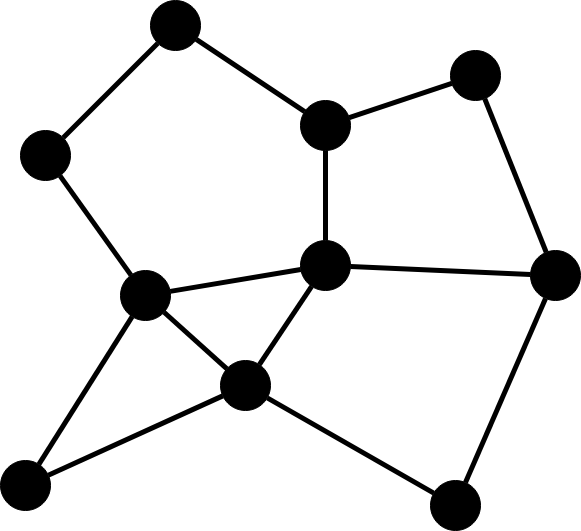
\includegraphics[scale=.4]{meshnet}
   \caption{Example of an \ac{IEEE} 802.11s mesh network}\label{fig:meshnet}
\end{figure}

The layer 2 routing protocol defined by \ac{IEEE} 802.11s that is used to create
and destroy these links is known as \ac{HWMP}~\cite{ieee80211}. In this
protocol, each station discovers other stations and manages a table of its
existing connections through a usage of the peer link management protocol, where
a station transmits beacons (frames with information about a network), and other
listening stations that want to become members of the same mesh network reply to
these transmissions. The table used to store these connections keeps not only
the direct connections the station has, but also the connections to stations
that are farther away, keeping an additional \textbf{nexthop} value, which holds
the address of the station that is directly connected to the source that
provides the best path to the destination, as seen in \autoref{fig:nexthop}. As
the name suggests, this protocol is hybrid, and it consists of two main
components. A proactive protocol, which is a tree-based hierarchical routing
protocol, and a reactive protocol, which is a modification of the
\ac{AODV}~\cite{aodv} routing protocol~\cite{ieee80211s}.

The proactive protocol works by having a station act as a designated root node,
and is only used when stations want to communicate with the root node or with
devices outside the mesh network~\cite{hwmpproa,hwmpperf}. When stations need to
communicate with other stations in the mesh network, the reactive protocol is
used. In this protocol, when a station needs to communicate with another, it
broadcasts a \textbf{Path Request} message with the \ac{MAC} address of the
destination. Intermediary stations rebroadcast this message while keeping
information from the transmitter of the message, in order to reach back with the
response. When the destination receives it, it updates its path to the source
and sends back a \textbf{Path Reply} in unicast~\cite{hwmpperf}.

\begin{figure}[htb]
   \centering
   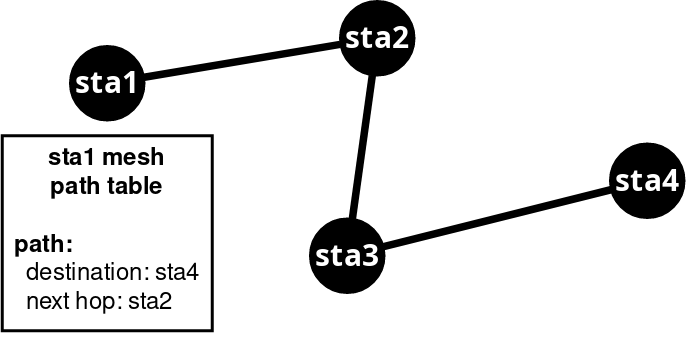
\includegraphics[scale=.4]{nexthop}
   \caption{Example of a mesh path}\label{fig:nexthop}
\end{figure}

In the Linux kernel's implementation of the data link layer for \ac{IEEE}
802.11s mesh networks, the connections between stations are known as
\textbf{mesh paths}, and the table where each system tracks these connections is
referred to as the \textbf{mesh path table}.


\section{eBPF}

The \ac{BPF} started out, as the name would suggest, as a packet filtering tool,
used only to accept or reject packets. This tool was created because the
existing packet filters were inefficient, having been developed for older
hardware. \ac{BPF} not only changed the design of the filter evaluator used,
replacing the stack-based one used by the original Unix packet filter with a
register-based evaluator, but it also changed the buffering strategy, resulting
in improved performance, among other things~\cite{bpf}.

\ac{BPF} filters packets using a directed acyclic control flow graph, where
nodes represent packet field predicates, and edges are control transfers. So,
for example, nodes would have checks in the form of "ether.type=IP", and edges
would be either a "yes" or a "no", with the flow going along the path of the
correct result. This approach is quite efficient, as it allows a \ac{BPF}
program to create a single flow graph that passes through several predicates,
having to parse each packet a single time, and ends in either a ``True'' or
``False'', deciding whether a packet should be processed or not, as seen in the
example in \autoref{fig:bpfprog}~\cite{bpf}. These filters can be written by
system administrators, and then run inside the Linux kernel, which allows
\ac{BPF} to check the packets before they are processed by the kernel.

\begin{figure}[htb]
   \centering
   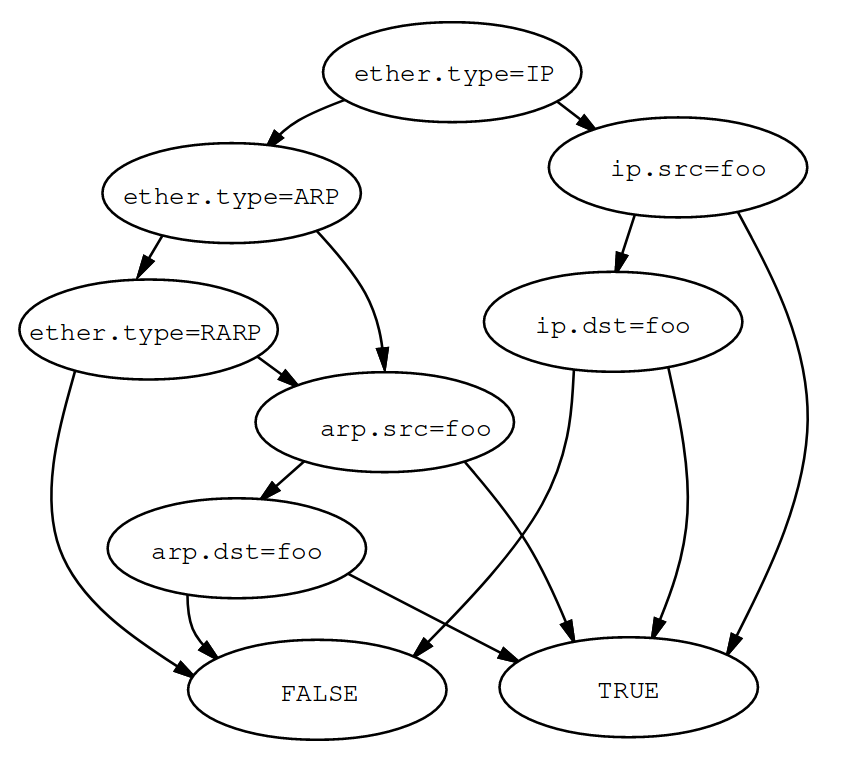
\includegraphics[scale=.3]{bpfprog}
   \caption{Example of a BPF program (Source:~\cite{bpf})}\label{fig:bpfprog}
\end{figure}

Seeing the potential of being able to write programs to run inside the kernel,
Alexei Starovoitov decided to improve \ac{BPF}, creating eBPF~\cite{alexei},
which used to be an acronym for ``extended BPF'', although that is no longer the
case~\cite{ebpfio}. Instead of simple flow-chart-like programs that can only be
used for packet filtering, eBPF now allows users to write more complex programs
that can involve arithmetic, structures, and pointers.

eBPF programs are executed on events, like function calls and network events,
through the use of, for example, \textbf{probes}, which are programs inserted
dynamically at the beginning or end of functions, which can be seen in
\autoref{fig:syscall}, with \textbf{kprobes} being used for functions inside the
kernel, and \textbf{uprobes} for functions in user-space, as well as
\textbf{tracepoints}, which are static points already present in the kernel
introduced by the kernel developers. These programs are loaded into the kernel
with the \texttt{bpf} system call and then pass through a verifier that ensures
that they are safe to run and do not get stuck in loops, checking if there are
any unreachable instructions, infinite loops, or instructions that harm the
system. Naturally, the verifier introduces some limitations to eBPF programs,
such as a limited number of instructions per eBPF program (Linux version 5.2
increased this number from 4096 to one million~\cite{sizelimit}), disallowing
conditional loops, and requiring root privileges for most programs~\cite{lwm}.
Finally, these programs are passed onto a \ac{JIT} compiler that optimises their
performance by translating the code into machine specific instructions. Also,
because eBPF is part of the Linux kernel, there is no need for external modules
to be installed to run these programs~\cite{ebpfio}.


\begin{figure}[htb]
   \centering
   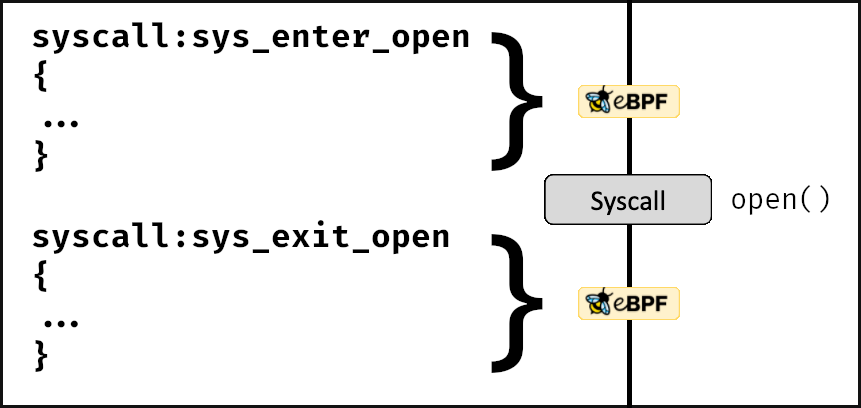
\includegraphics[scale=.35]{syscall}
   \caption{Example of eBPF tracepoints}\label{fig:syscall}
\end{figure}

eBPF also introduces mechanisms to help with development. Probes have already
been mentioned, but it also provides BPF maps, which allow programs to save data
temporarily in kernel-space, enabling sharing of information across probes and
to user-spaced~\cite{lwm}.

Not only that, but eBPF can also be used to write \ac{XDP} programs. \ac{XDP} is
a framework that allows for processing packets at the lowest possible level,
even before the kernel itself can process them. Some network cards even support
using \ac{XDP} in the controller itself, allowing for super fast processing of
packets. This, however, has limitations as well, since the programs are written
in a restricted variant of C, because they need to be translated into eBPF
byte-code, and \ac{XDP} can only be used in packet reception~\cite{xdp}.

eBPF has become an important tool in the last few years, especially in the area
of networks, having been used for discovery of dependencies in network
services~\cite{ebpfeg1}, taking advantage of its small performance overhead, as
well as monitoring traffic in Open vSwitches~\cite{ebpfeg2}, proving to be a
better choice against other monitoring solutions thanks to its code verifier,
which ensures that buggy eBPF code will not crash or otherwise severely
interfere with a system.


\section{BCC}

The \ac{BCC} is a toolkit with the purpose of allowing the creation of eBPF
programs more easily, with front-ends in both Lua and Python. This tool allows
for easier development of eBPF programs, as it abstracts the use of the \ac{BPF}
system call, replacing this with C-like code, which is then loaded into the
system with calls from a Python or Lua program. The toolkit is well documented,
and it also comes with some pre-made programs, which serve as examples of useful
eBPF programs~\cite{gregg,bcc}.

The ease of use comes at a cost, however, as \ac{BCC} embeds the LLVM toolchain
to compile programs, which leads to heavy processor and memory usage on
compilation~\cite{pingcap,contain}. This can become a problem since \ac{BCC}
compiles programs every time they are run. Not only that, but \ac{BCC} also
requires the system to have the kernel header packages installed, which not only
occupies extra space on the system to hold these
packages~\cite{pingcap,contain}, but can also be problematic, especially when
working with multiple Linux distributions, where the kernel header packages'
content can be different, which is exactly one of the problems we faced in
\autoref{sect:mac802}.

BCC used to be the primary choice for development of complex eBPF programs, but
it is now considered deprecated, with newer programs using libbpf together with
\ac{CO-RE}~\cite{toolsfuture}.


\section{bpftrace}

IO Visor, the project behind \ac{BCC}, has also introduced bpftrace, which is a
high-level language for tracing the Linux kernel that uses eBPF~\cite{bpftrace}.
Unlike \ac{BCC}, it is not a library, so no extra code is needed to run
programs. The user can simply write their bpftrace program and execute it
directly with the \texttt{bpftrace} command. However, it does not have an API
that allows for manipulation of data outside bpftrace. Also, like \ac{BCC},
bpftrace needs the kernel header packages for structure and other type
definitions~\cite{bpftrace}.

Due to being less verbose than \ac{BCC}, bpftrace is much easier to work with,
but because of its lack of API, which only allows to send information to the
standard output, it becomes useful only for programs that do not need to send
data to user-space. Still, if data needs to sent to user-space, bpftrace is
still useful for small tests and to quickly find all the available probes and
tracepoints through the usage of its \texttt{-l} flag, which lists all probes.


\section{perf}

perf is a Linux command used to analyse the Linux kernel's performance. perf
provides several subcommands that can record events, count the number of events
in a given timeframe, see events in real time, etc~\cite{perf}. perf was
originally created before eBPF, but it now uses it for tracing with tracepoints
and probes~\cite{greggperf}, and eBPF itself uses perf, for example, to send
data from BPF maps to user-space using perf buffers~\cite{perfring}.

perf is very similar to bpftrace, and like it, it is most suitable for smaller
scripts instead of big applications, suffering from the same disadvantages as
bpftrace.


\section{libbpf}

libbpf is a library written in C/C++ designed to allow loading and interacting
with eBPF programs~\cite{libbpf}. It is considered an alternative to \ac{BCC},
but with many advantages over it. libbpf abstracts many aspects of eBPF, just
like \ac{BCC}, but, unlike \ac{BCC}, which compiles the eBPF programs at
runtime, libbpf allows programs to be compiled into eBPF
bytecode~\cite{libbpf,contain}, eliminating the need of several dependencies on
the system in which the programs are being executed. Not only that, but libbpf
doesn't rely on kernel headers, instead using a header file that contains
multiple kernel structure definitions and types, eliminating the need for kernel
headers to be installed on the system~\cite{contain}. The drawback is that it is
not as well documented as \ac{BCC}, having almost only examples to serve as aid
in development.


\subsection{CO-RE}

\ac{CO-RE} is an approach implemented by libbpf that allows the creation of
portable eBPF programs, meaning that programs only need to be compiled once, and
can then be deployed across multiple systems, working even if these systems
differ in architecture and kernel version~\cite{coreref,fbslide}. This is
possible because of the \ac{BTF}. \ac{BTF} is a format that encodes debug
information, akin to \ac{DWARF}, but in a more compact and efficient manner, and
is used to provide information like structure offsets, which can then be used by
\ac{CO-RE} to relocate the eBPF bytecode as needed by the kernel version being
used~\cite{core}. This means that the kernel needs to be compiled with support
for \ac{BTF}. Thankfully, because \ac{BTF} support only amounts to about 1.5
megabytes in increase to the kernel image, most distributions already compile
their kernels for x86 architectures with the support~\cite{toolsfuture}.
Similarly to \ac{BCC}, a program needs to be created in order to load eBPF
programs, but \ac{CO-RE} also requires a file containing the structures and type
definitions used in the kernel to be generated (although this only needs to be
done once)~\cite{bootstrap}.

The problem with \ac{CO-RE} is pretty much the same as libbpf: it is not well
documented, and most of its documentation consists of a few blog posts made by
its main developer. The blog posts are actually quite well written, but they
only touch on the general uses of elements from \ac{CO-RE} with a few examples.
For more specific questions a developer might have, they are not very helpful.

Although libbpf and \ac{CO-RE} are recent technologies, they are used by big
companies like Facebook (where \ac{CO-RE} was created)~\cite{fbslide}, as well
as in projects for monitoring networks of Kubernetes clusters~\cite{kuber} and
security of Linux-based containers~\cite{sec}.
